
%(BEGIN_QUESTION)
% Copyright 2015, Tony R. Kuphaldt, released under the Creative Commons Attribution License (v 1.0)
% This means you may do almost anything with this work of mine, so long as you give me proper credit

\noindent
{\bf Lab Exercise -- introduction}

\vskip 5pt

Your team's task is to construct a three-phase reversing motor starter circuit, complete with a transformer bank to convert 480 VAC power to 240 VAC or 208/120 VAC power.  You will also demonstrate proper safety precautions appropriate for working with three-phase power circuitry, including lock-out-tag-out and verification of safe conditions using a multimeter.

The following table of objectives show what you and your team must complete within the scheduled time for this lab exercise.  Note how some of these objectives are individual, while others are for the team as a whole:

\underbar{Objective completion table:}

% No blank lines allowed between lines of an \halign structure!
% I use comments (%) instead, so that TeX doesn't choke.

$$\vbox{\offinterlineskip
\halign{\strut
\vrule \quad\hfil # \ \hfil & 
\vrule \quad\hfil # \ \hfil & 
\vrule \quad\hfil # \ \hfil & 
\vrule \quad\hfil # \ \hfil & 
\vrule \quad\hfil # \ \hfil & 
\vrule \quad\hfil # \ \hfil & 
\vrule \quad\hfil # \ \hfil \vrule \cr
\noalign{\hrule}
%
% First row
{\bf Performance objective} & {\bf Grading} & {\bf 1} & {\bf 2} & {\bf 3} & {\bf 4} & {\bf Team} \cr
%
\noalign{\hrule}
%
% Another row
Team meeting and prototype sketch (do {\it first!}) & mastery & -- & -- & -- & -- & \cr
%
\noalign{\hrule}
%
% Another row
Circuit design challenge & mastery & & & & & -- -- -- -- \cr
%
\noalign{\hrule}
%
% Another row
Final schematic diagram and system inspection & mastery & & & & & -- -- -- -- \cr
%
\noalign{\hrule}
%
% Another row
Proper use of insulation tester & mastery & & & & & -- -- -- -- \cr
%
\noalign{\hrule}
%
% Another row
Safety demonstrations & mastery & & & & & -- -- -- -- \cr
%
\noalign{\hrule}
%
% Another row
Hazard/risk assessment as per NFPA 70E & mastery & -- & -- & -- & -- &  \cr
%
\noalign{\hrule}
%
% Another row
Transformer bank wiring inspection & mastery & -- & -- & -- & -- &  \cr
%
\noalign{\hrule}
%
% Another row
Proper motor control function & mastery & -- & -- & -- & -- &  \cr
%
\noalign{\hrule}
%
% Another row
Troubleshooting & mastery & & & & & -- -- -- -- \cr
%
\noalign{\hrule}
%
% Another row
Lab question: Wiring connections & proportional &  &  &  &  & -- -- -- -- \cr
%
\noalign{\hrule}
%
% Another row
Lab question: Commissioning & proportional &  &  &  &  & -- -- -- -- \cr
%
\noalign{\hrule}
%
% Another row
Lab question: Mental math & proportional &  &  &  &  & -- -- -- -- \cr
%
\noalign{\hrule}
%
% Another row
Lab question: Diagnostics & proportional &  &  &  &  & -- -- -- -- \cr
%
\noalign{\hrule}
%
% Another row
Decommission and lab clean-up & mastery & -- & -- & -- & -- &  \cr
%
\noalign{\hrule}
%
% Another row
Personal tool kit complete (show on last day) & mastery &  &  &  &  & -- -- -- -- \cr
%
\noalign{\hrule}
%
% Another row
Reply to email message on BTC account & mastery &  &  &  &  & -- -- -- -- \cr
%
\noalign{\hrule}
} % End of \halign 
}$$ % End of \vbox

The only ``proportional'' scoring in this activity are the lab questions, which are answered by each student individually.  A listing of potential lab questions are shown at the end of this worksheet question.  The lab questions are intended to guide your labwork as much as they are intended to measure your comprehension, and as such the instructor may ask these questions of your team day by day, rather than all at once (on a single day).

\vskip 10pt

In addition to this motor control system, you must individually construct a {\it PLC trainer} for learning PLC programming.  An example is documented in the next question of this worksheet.

\underbar{PLC objective completion table:}

% No blank lines allowed between lines of an \halign structure!
% I use comments (%) instead, so that TeX doesn't choke.

$$\vbox{\offinterlineskip
\halign{\strut
\vrule \quad\hfil # \ \hfil & 
\vrule \quad\hfil # \ \hfil & 
\vrule \quad\hfil # \ \hfil & 
\vrule \quad\hfil # \ \hfil & 
\vrule \quad\hfil # \ \hfil & 
\vrule \quad\hfil # \ \hfil & 
\vrule \quad\hfil # \ \hfil \vrule \cr
\noalign{\hrule}
%
% First row
{\bf Performance objective} & {\bf Grading} & {\bf 1} & {\bf 2} & {\bf 3} & {\bf 4} & {\bf Team} \cr
%
\noalign{\hrule}
%
% Another row
All components unwired before construction & mastery & & & & & -- -- -- -- \cr
%
\noalign{\hrule}
%
% Another row
All inputs (switches) function properly & mastery & & & & & -- -- -- -- \cr
%
\noalign{\hrule}
%
% Another row
All outputs (lights) function properly & mastery & & & & & -- -- -- -- \cr
%
\noalign{\hrule}
} % End of \halign 
}$$ % End of \vbox

{\bf It is essential that your team plans ahead what to accomplish each day.  A short (10 minute) team meeting at the beginning of each lab session is a good way to do this, reviewing what's already been done, what's left to do, and what assessments you should be ready for.  There is a lot of work involved with building, documenting, and troubleshooting these working instrument systems!}

As you and your team work on this system, you will invariably encounter problems.  You should always attempt to solve these problems as a team before requesting instructor assistance.  If you still require instructor assistance, write your team's color on the lab whiteboard with a brief description of what you need help on.  The instructor will meet with each team in order they appear on the whiteboard to address these problems.




\vfil \eject







\noindent
{\bf Lab Exercise -- team meeting, prototype sketch, and instrument selection}

\vskip 5pt

An important first step in completing this lab exercise is to {\bf meet with your instructor} as a team to discuss safety concerns, team performance, and specific roles for team members.  If you would like to emphasize exposure to certain equipment (e.g. use a particular type of control system, certain power tools), techniques (e.g. fabrication), or tasks to improve your skill set, this is the time to make requests of your team so that your learning during this project will be maximized.

\vskip 10pt

An absolutely essential step in completing this lab exercise is to work together as a team to {\bf sketch a prototype diagram} showing what you intend to build.  This usually takes the form of a simple electrical schematic and/or loop diagram showing all electrical connections between components, as well as any tubing or piping for fluids.  This prototype sketch need not be exhaustive in detail, but it does need to show enough detail for the instructor to determine if all components will be correctly connected for their safe function.

For example, if you intend to connect field devices to a PLC (Programmable Logic Controller), your prototype sketch must show how those devices will connect to typical input/output terminals on the PLC, where electrical power will be supplied, etc.  Prototype sketches need not show all intermediary connections between components, such as terminal blocks in junction boxes between the field device and the controller.

You should practice good problem-solving techniques when creating your prototype sketch, such as consulting equipment manuals for information on component functions and marking directions of electric current, voltage polarities, and identifying electrical sources/loads.  Use this task as an opportunity to strengthen your analytical skills!  Remember that you will be challenged in this program to do all of this on your own (during ``capstone'' assessments), so do not make the mistake of relying on your teammates to figure this out for you -- instead, treat this as a problem {\it you} must solve and compare your results with those of your teammates.

Your team's prototype sketch is so important that the instructor will demand you provide this plan before any construction on your team's working system begins.  {\it Any team found constructing their system without a verified plan will be ordered to cease construction and not resume until a prototype plan has been drafted and approved!}  Similarly, you should not deviate from the prototype design without instructor approval, to ensure nothing will be done to harm equipment by way of incorrect connections.  Each member on the team should have ready access to this plan (ideally possessing their own copy of the plan) throughout the construction process.  Prototype design sketching is a skill and a habit you should cultivate in school and take with you in your new career.

\vskip 10pt

When selecting components for this lab exercise, you will need to choose a step-down ``control power'' transformer, a pair of three-phase contactors (one for forward and one for reverse), and an overload ``heater'' assembly.  A three-pushbutton Forward/Reverse/Stop control station has already been constructed for you, having four wires ready to connect to your motor starter assembly:

$$\includegraphics[width=15.5cm]{i02132x09.eps}$$

After locating suitable components, you should qualitatively test them prior to construction of your system.  For an electric motor, this means checking continuity through all the windings.  For switches, ohmmeter (``continuity'') measurements will tell you if the switch contacts are actuating as they should.  For the contactor, you may manually actuate the contacts and also check the contacts and coil for continuity using your ohmmeter.  If any component fails to respond properly, notify the instructor and then tag it with a label explaining what it does (or what it fails to do).

\vskip 10pt

Another detail important to the planning of your system is identifying the necessary gauge (size) of the wires used.  Consult article 310 of the National Electrical Code (the ``NEC,'' also known as {\it NFPA 70}) book regarding ``ampacity'' ratings for different gauges of stranded copper wire.  Your motor's nameplate will provide the information you will need on line current.

\vskip 10pt

{\bf Planning a functioning system should take no more than an hour if the team is working efficiently, and will save you hours of frustration (and possible component destruction!).}







\vfil \eject

\noindent
{\bf Lab Exercise -- circuit design challenge}

\vskip 5pt

Connect an ``ice-cube'' relay to a low-voltage DC source as well as 120 volts AC so that a hand-operated switch will control the energization of a 120 VAC load.  All electrical connections must be made using a terminal strip (no twisted wires, crimp splices, wire nuts, spring clips, or ``alligator'' clips permitted), and the 120 VAC portion of the circuit must be fused for overcurrent protection.

This exercise tests your ability to properly interpret the ``pinout'' of an electromechanical relay, properly wire a switch to control a relay's coil, properly wire a load to the contacts of a relay, properly select NO/NC contacts on both the switch and the relay, and use a terminal strip to organize all electrical connections.

$$\includegraphics[width=15.5cm]{i02132x06.eps}$$

\vskip 10pt

The following components and materials will be available to you: assorted ``ice cube'' {\bf relays} with DC-rated coils and matching {\bf sockets} ; assorted pushbutton {\bf switches} ; {\bf terminal strips} ; lengths of {\bf hook-up wire} ; {\bf battery clips} (holders) ; 120 VAC {\bf power cord} with {\bf fuse assembly} ; 120 VAC {\bf lamp or other suitable load}.

\vskip 10pt

You will be expected to supply your own screwdrivers and multimeter for assembling and testing the circuit at your desk.  The instructor will supply the battery(ies) to power your circuit when you are ready to see if it works.  Until that time, your circuit will remain unpowered.

\vskip 20pt

\noindent
{\bf Load/switch status} (instructor chooses): \hskip 20pt \underbar{\hskip 20pt} On when pressed \hskip 10pt {\it or} \hskip 10pt \underbar{\hskip 20pt} Off when pressed

\vfil

Study reference: the ``Control Relays'' section of {\it Lessons In Industrial Instrumentation}.









\vfil \eject

\noindent
{\bf Lab Exercise -- documenting the system}

\vskip 5pt

Given the hazards associated with three-phase AC power circutry, it is essential that you carefully plan your circuit in its entirety prior to assembling it.  For this reason, the instructor will require a complete, detailed schematic diagram of your motor starter circuit.  These diagrams must be thoroughly checked for accuracy and electrical safety, to ensure no unnecessary hazards are present when power is applied.

\vskip 10pt

A sample schematic diagram for a one-direction motor starter circuit is shown on the next page.  Your schematic diagram must be {\it comprehensive} and {\it detailed}, showing every wire connection, every cable, every terminal block, etc.  The principle to keep in mind here is to make the schematic diagram so complete and unambiguous that anyone can follow it to see what connects to what, even someone unfamiliar with motor control circuits.  In industry, systems are often constructed by contract personnel with limited understanding of how the system is supposed to function.  The schematic diagrams they follow must be so complete that they will be able to connect everything properly without necessarily understanding how it is supposed to work.

Note that each and every wire in your system needs to be labeled with a number.  Wires electrically common to each other at all times (i.e. connected at terminal blocks, not passing through any component) must bear the same label number.  An easy way to label wires is to wrap a short piece of masking tape around each wire then writing on that masking tape with a permanent marker.  Furthermore, each number or other label appearing on a device terminal (e.g. the screw terminals on an octal-base relay socket) must be shown on your schematic diagram in parentheses, to distinguish those labels from wire numbers used to identify wires.  With each wire and each device terminal clearly labeled, one cannot go wrong in re-connecting wires that were undone.  This is important when technicians remove components for repair and replacement, as the schematic diagram is their only guide to proper re-connection of the new or repaired components.

When your entire team is finished drafting your individual schematic diagrams, call the instructor to do an inspection of the system.  Here, the instructor will have students take turns going through the entire system, with the other students checking their diagrams for errors and omissions along the way.  During this time the instructor will also inspect the quality of the installation, identifying problems such as frayed wires, improperly crimped terminals, poor cable routing, missing labels, lack of wire duct covers, etc.  The team must correct all identified errors in order to receive credit for their system.  

After successfully passing the inspection, each team member needs to place their schematic diagram in the diagram holder located in the middle of the lab behind the main control panel.  When it comes time to troubleshoot another team's system, this is where you will go to find a schematic diagram for that system!

\filbreak

Note that this sample diagram is shown only to illustrate the conventions you should use in documenting wire labels, terminal labels, etc.  Your team's diagram will differ substantially from this one, most notably because it is a reversing motor control circuit whereas this example diagram shows a one-directional motor control circuit:

$$\includegraphics[width=15.5cm]{i02132x02.eps}$$  % schematic diagram for a one-direction motor starter circuit

Reversing motor control circuits always contain normally-closed {\it interlocking} relay contacts to prevent simultaneous energization of both ``Forward'' and ``Reverse'' contactors.  The one-direction motor control circuit shown above lacks interlock contacts, because there is only one direction it can turn.

Feel free to consult the ``Typical Wiring Diagrams'' booklet produced by Allen-Bradley for manual and magnetic full-voltage starter units, contained on your Instrumentation Reference.  This booklet shows a wide variety of starter circuit configurations, including diagrams for reversing starter circuits.

Note that wiring diagrams for motor control circuits often take two forms: {\it schematic} and {\it pictorial}.  Schematic diagrams are laid out in such a way as to minimize the number of wire crossings, in order to aid visual analysis of the circuit.  Pictorial diagrams, on the other hand, are laid out in a manner resembling the physical orientation of circuit components, and therefore typically are more difficult to analyze because there are many more wires crossing over each other in order to reach their intended terminal points.  It is highly recommended that you make your diagrams {\it schematic} rather than pictorial, especially for ease of interpretation when you do troubleshooting on motor control circuits and must use the diagram to determine your diagnostic tests.



\vskip 10pt

{\bf Common mistakes:}

\begin{itemize}
\item{} Copying (verbatim) a sample diagram from a book, rather than customizing the diagram for the components at hand.
\item{} Basing your diagram off of a team-mate's diagram, rather than closely inspecting the system for yourself.
\item{} Forgetting to label all wires (see example diagram).
\item{} Forgetting to label all terminals (see example diagram).
\item{} Forgetting to note all wire colors.
\item{} Forgetting to put your name on the schematic diagram!
\end{itemize}

\vskip 10pt

{\bf Creating and inspecting accurate schematic diagrams should take no more than one full lab session (3 hours) if the team is working efficiently!}

\filbreak


%\centerline{\bf Pictorial diagram template}

%$$\includegraphics[width=15.5cm]{i02132x04.eps}$$  % pictorial diagram for a one-direction motor starter circuit

%Note that your pictorial diagram should show the respective components {\it exactly} as they are arranged on your team's panel, not necessarily as they appear in this example template.






\vfil \eject

\noindent
{\bf Lab Exercise -- building the system}

\vskip 5pt

After getting your wiring diagram approved by the instructor, you are cleared to begin building your system.  Mount all control components (control power transformer, contactors, overload unit, fuse holders) on a metal subpanel (plate) designed to insert into an electrical enclosure.  Locate the pushbutton switched at some other location such as the main control panel for the lab.  This ensures a long enough cable run for the switches to make the system realistic for testing and troubleshooting.  Note: you must marshall all switch wiring through terminal blocks on the subpanel, so that the switches may be disconnected from the rest of the control circuit without disturbing any other wiring.

Power to your control circuit will come through four terminals located at one edge of the metal subpanel: three fused terminals for the three-phase power lines (L1, L2, and L3), and one unfused terminal for earth (safety) ground which will be bonded to the metal subpanel.  Plastic ``wire duct'' will be used to route all wires between components.  Here is a model layout (note that yours may look different):

$$\includegraphics[width=15.5cm]{i02132x01.eps}$$

All wires need to enter and exit the wire duct perpendicularly for a neat and professional appearance.  All conductors must be stranded copper, of sufficient gauge for the full-load motor current according to the National Electrical Code (NEC).  Each wire should bear its number label at each end where it terminates.

\vskip 10pt

Before applying power to your motor control starter circuit, it must be inspected under instructor supervision.  Testing will be performed using a high-voltage insulation tester (sometimes called a ``Megger'' in honor of a proper brand name for this type of instrument) to check for proper connections, proper fuse operation (i.e. when a fuse is pulled out of its socket, continuity to the protected device is interrupted), etc. 

\vskip 10pt

{\bf Common mistakes:}

\begin{itemize}
\item{} Failing to tug on each and every wire where it terminates to ensure a mechanically sound connection.
\item{} Students working on portions of the system in isolation, not sharing with their teammates what they did and how.  It is important that the whole team learns all aspects of their system!
\end{itemize}

\vskip 10pt

{\bf Building a functioning system should take no more than one full lab session (3 hours) if all components are readily available and the team is working efficiently!}








\vfil \eject

\noindent
{\bf Lab Exercise -- insulation tester usage}

\vskip 5pt

An {\it insulation tester} is a special kind of ohmmeter designed to detect high-resistance paths for electric current (in the hundreds of megaohms).  The purpose of using an insulation tester when checking the integrity of electric motors and motor control circuits is to reveal any breakdowns of electrical insulation that might not otherwise be detected using a regular low-range ohmmeter.

What makes an insulation tester different from a regular ohmmeter is its use of relatively high voltage to perform the test.  Unlike a regular ohmmeter which only applies a few volts (or even just a few tenths of a volt for many modern DMM ohmmeter functions) to the circuit under test, an insulation tester contains within it a high-voltage generator capable of supplying hundreds or even thousands of volts to the test leads in order to ``stress'' the circuit under test and reveal any breakdown of insulation.  This makes an insulation tester capable of delivering an electrical shock to the user if incorrectly operated!

Legacy insulation testers, especially the ``Megger'' brand whose name has become synonymous with insulation test instruments, used hand-crank electromechanical generators to create this high voltage.  Early ``Megger'' testers actually had a small crank handle protruding from the side which the user would turn after having connected the test leads to the circuit.  If something went wrong and the user became shocked by the tester's output voltage, they would naturally stop cranking the handle.  Modern insulation testers have battery-powered high voltage generator circuits, and use a pushbutton to trigger the application of high voltage to the circuit under test.  Again, the notion being that anyone shocked by the output of the instrument will naturally stop pressing the button.

All insulation testers have rather high output impedance, so that when connected across a short-circuit the high-voltage power source inside the tester will not be damaged by excessive current.  This makes insulation testers perfectly valid for testing continuity in addition to testing for the presence of non-continuity (i.e. that conductors are insulated from each other).

\vskip 10pt

Most insulation testers provide a way to vary the amount of voltage output by the tester, for different testing applications.  When using an insulation tester, you want to use a test voltage greater than that normally experienced by the device or circuit under test, in order to adequately ``stress'' that device or circuit to ensure its proper operation when energized by its normal supply voltage.  However, you do not want to use so much voltage that you actually cause damage to the device or circuit under test!  This means the tester's output voltage should be configured to be {\it just one step above the circuit's normal operating voltage}.

Devices most susceptible to damage from mis-use of an insulation tester are {\it semiconducting} in nature.  Diodes, transistors, SRCs, TRIACs, and associated devices may all be damaged rather easily by the mis-application of an insulation tester.  This means one should not use an insulation tester on a circuit containing complex and expensive semiconductor components such as variable-speed motor drives (VSDs or VFDs).  








\vfil \eject

\noindent
{\bf Lab Exercise -- safety demonstrations}

\vskip 5pt

This lab exercise, more than any other, harbors a significant level of personal danger due to the use of 480 VAC power.  Exercising safe work habits is not just an objective of this lab, but it is essential for avoiding injury!  This lab requires you to demonstrate the following procedures:

\begin{itemize}
\item{} The one-hand rule (working only with your right hand -- keeping the left hand in a pocket or behind your back -- when working on any energized circuit)
\vskip 10pt
\item{} Lock-out, Tag-out (properly documenting work to be done on a tag, then attaching both tag and lock to the disconnect device securing power)
\vskip 10pt
\item{} Attempt to start the motor (as a crude check to see that power has been disconnected)
\vskip 10pt
\item{} Proper use of meter to check for dangerous voltage (check for voltage between all possible pairs of points -- including earth ground -- and then verifying the meter's operation against a known voltage source)
\end{itemize}











\vfil \eject

\noindent
{\bf Lab Exercise -- hazard/risk assessment}

\vskip 5pt

Here, you will work with your team to perform an assessment of hazards and risks posed by a particular job assignment selected by your instructor.  Your assessment needs to be based on the NFPA 70E ``Standard for Electrical Safety in the Workplace'' document.  Your assessment shall account for arc flash as well as for electric shock, and will detail necessary PPE (Personal Protective Equipment) and procedures necessary for safe work.

Your instructor will randomly select a job task.  Examples include:

\begin{itemize}
\item{} Attaching 4-20 mA wires to the back of a panel-mounted loop controller while the controller is powered by 120 VAC.
\vskip 5pt
\item{} Using a multimeter to take voltage measurements on a 208 VAC motor starter circuit while it is powered through the step-down transformer bank.
\vskip 5pt
\item{} Using a multimeter to take voltage measurements on the 480 VAC lines feeding the step-down transformer bank.
\vskip 5pt
\item{} Using a multimeter to take voltage measurements on a live 480 VAC motor starter circuit fed directly from a three-phase transformer with a specified MVA rating.
\vskip 5pt
\item{} Using a multimeter to take voltage measurements on a VFD while it is powered through an isolation transformer of specified KVA rating (just like some of the VFDs in our lab).
\vskip 5pt
\item{} ``Racking in'' a 4160 VAC circuit breaker into a live panel.
\vskip 5pt
\item{} Using a clamp-on ammeter to measure current through a line feeding a 480 VAC motor.
\end{itemize}

\vskip 10pt

Here are some details which must be included in your final assessment of hazards and risks:


\begin{itemize}
\item{} Arc flash boundary distance = \underbar{\hskip 50pt} inches
\vskip 5pt
\item{} Necessary arc flash protective clothing to wear = \underbar{\hskip 50pt}
\vskip 5pt
\item{} Approach distance for a qualified worker = \underbar{\hskip 50pt} inches 
\vskip 5pt
\item{} Necessary gloves to wear = \underbar{\hskip 50pt}
\vskip 5pt
\item{} Whether or not electrically insulated tools are required
\vskip 5pt
\item{} {\it Citations showing where in NFPA 70E you obtained the information}
\end{itemize}
















\vfil \eject

\noindent
{\bf Lab Exercise -- wiring the step-down transformer bank}

\vskip 5pt

In order to power your 240 VAC or 208 VAC motor from the 480 VAC receptacle in the lab, you will need to wire three transformers together to create a three-phase transformer bank.  Here are your configuration options, based on the different possible primary/secondary voltage ratings available for the transformers:

$$\includegraphics[width=15.5cm]{i02132x03.eps}$$  % transformer bank configurations

You may have multiple options available to you, depending on the rating of your motor and the particular transformers used to for the three-phase bank.  If this is the case, your instructor will choose one of the configurations for you.

\vskip 10pt

After this, you must work as a team to determine the proper phasing (``polarity'') for the transformers and then connect the necessary wires in order to build the desired circuit.  You may find the section titled ``Transformer Polarity'' in your {\it Lessons In Industrial Instrumentation} textbook helpful in explaining this concept.  The instructor must inspect your plan as well as the constructed circuit before you are allowed to apply power to the transformer bank.

\vfil \eject

The following pictorial diagram might be useful for you and your team to use for sketching the necessary Delta/Wye connections and transformer winding jumpers to achieve the necessary step-down ratios:

$$\includegraphics[width=15.5cm]{i02132x05.eps}$$  % transformer pictorial diagram








\vfil \eject

\noindent
{\bf Lab Exercise -- troubleshooting}

\vskip 5pt

The most challenging aspect of this lab exercise is {\it troubleshooting}, where you demonstrate your ability to logically isolate a problem in the system.  All troubleshooting is done on an individual basis (no team credit!), and must be done {\it on a system you did not help build}, so that you must rely on schematic diagrams to find your way around the system instead of from your own memory of building it.

Each student is given a limited amount of time to identify both the general location and nature of the fault, logically justifying all diagnostic steps taken.  All troubleshooting activities will take place under direct instructor supervision to ensure students are working independently and efficiently. 

Failure to correctly identify both the general location and nature of the fault within the allotted time, and/or failing to demonstrate rational diagnostic procedure to the supervising instructor will disqualify the effort, in which case the student must re-try with a different fault.  Multiple re-tries are permitted with no reduction in grade.

A standard multimeter is the only test equipment allowed during the time limit.  No diagnostic circuit breaks are allowed except by instructor permission, and then only after correctly explaining what trouble this could cause in a real system.  

The instructor will review each troubleshooting effort after completion, highlighting good and bad points for the purpose of learning.  Troubleshooting is a skill born of practice and failure, so do not be disappointed in yourself if you must make multiple attempts to pass!  One of the important life-lessons embedded in this activity is how to deal with failure, because it {\it will} eventually happen to you on the job!  There is no dishonor in failing to properly diagnose a fault after doing your level best.  The only dishonor is in taking shortcuts or in giving up.

\vskip 10pt

{\bf Common mistakes:}

\begin{itemize}
\item{} Neglecting to take measurements with your multimeter.
\item{} Neglecting to check other measurements in the system (e.g. pressure gauge readings).
\item{} Incorrectly interpreting the wiring diagram (e.g. thinking you're at the wrong place in the system when taking measurements).
\item{} Incorrect multimeter usage (e.g. AC rather than DC, wrong range, wrong test lead placement).  This is especially true when a student comes to lab unprepared and must borrow someone else's meter that is different from theirs!
\end{itemize}

\vskip 10pt

{\bf Remember that the purpose of the troubleshooting exercise is to foster and assess your ability to intelligently diagnose a complex system.  Finding the fault by luck, or by trial-and-error inspection, is not a successful demonstration of skill.  The only thing that counts as competence is your demonstrated ability to logically analyze and isolate the problem, correctly explaining all your steps!}

\vskip 10pt

{\bf Troubleshooting takes a lot of lab time, usually at least two 3-hour lab sessions for everyone in a full class to successfully pass.  Be sure your team budgets for this amount of time as you plan your work, and also be sure to take advantage of your freedom to observe others as they troubleshoot, to better learn this art.}




\vfil \eject

\noindent
{\bf Lab questions}

\vskip 5pt

\begin{itemize}
\item{} {\bf Wiring connections}
\item{} Determine correct wire connections between components to create a working 3-phase motor control circuit, based on diagrams of components with terminals labeled
\end{itemize}

\filbreak

\begin{itemize}
\item{} {\bf Commissioning and Documentation}
\item{} Explain the meanings of the various ratings specified on a motor nameplate
\item{} Explain the meanings of the coil and contact ratings specified on a contactor nameplate
\item{} Explain how an {\it insulation tester} may be used to test the integrity of an electric motor's windings
\item{} Explain how an {\it insulation tester} might cause damage to circuit components if improperly used
\item{} Explain how to configure a multi-voltage induction motor for different operating voltages, given the information shown on a motor nameplate
\item{} Explain what {\it arc flash} and {\it arc blast} are, and what causes these effects
\item{} Explain how {\it overload heaters} in a motor control circuit perform a function fundamentally different from a fuse or a circuit breaker
\end{itemize}

\filbreak

\begin{itemize}
\item{} {\bf Mental math} (no calculator allowed!)
\item{} Convert horsepower rating of a three-phase AC electric motor into a current rating (at a specified line voltage)
\item{} Convert current rating of a three-phase AC electric motor into a horsepower rating (at a specified line voltage)
\end{itemize}

\filbreak

\begin{itemize}
\item{} {\bf Diagnostics}
\item{} Determine whether or not a given diagnostic test will provide useful information, given a set of symptoms exhibited by a failed system
\item{} Identify at least two plausible faults given the results of a diagnostic test and a set of symptoms exhibited by a failed system
\item{} Propose a diagnostic test for troubleshooting a failed system and then explain the meanings of two different test results
\end{itemize}


\vfil \eject

\noindent
{\bf Lab Exercise -- decommissioning and clean-up}

\vskip 5pt

The final step of this lab exercise is to decommission your team's entire system and re-stock certain components back to their proper storage locations, the purpose of which being to prepare the lab for the next lab exercise.  Remove your system documentation (e.g. wiring diagram) from the common holding area, either discarding it or keeping it for your own records.  Also, remove all wire labels from wiring and cables.

\vskip 10pt

\indent
{\bf Leave the following components in place, mounted on the racks:}

\begin{itemize}
\item{} Large electric motors
\item{} Large variable-frequency drive (VFD) units
\item{} Cables inside conduit interconnecting junction boxes together
\item{} Pipe and tube fittings (do not unscrew pipe threads)
\item{} Supply air pressure regulators
\end{itemize}

\vskip 10pt

\indent
{\bf Return the following components to their proper storage locations:}

\begin{itemize}
\item{} Manual (e.g. pushbutton) switches
\item{} ``Jumper'' cables used to connect terminal blocks within a single junction box
\item{} Power cables and extension cords
\end{itemize}













\vfil \eject

\noindent
{\bf Lab Exercise -- tool kit and email usage}

\vskip 5pt

Two additional objectives that are not technically a part of making this lab project function, but are nevertheless very important to your continued success in the Instrumentation program, include assembling a personal tool kit and using your BTC email account (which is automatically created for every student at the college).  

\vskip 10pt

You will be using your tool kit throughout the remainder of this program, and so it is very important to have it complete and ready to use by the end of this lab exercise.  Note that there are several optional items listed in addition to mandatory items.  These optional tools are useful, but not 100\% necessary for the work you will be doing in the lab.  Also note that there are some consumable items in your tool list such as electrical compression terminals which you will need to keep stocked as you use them in your labwork.

\vskip 10pt

Likewise, you will be relying on email to receive important messages from your instructor(s) throughout the remainder of the program.  These messages include, but are not limited to, job announcements, guest speaker appearances, schedule changes, emergency notifications, scholarship announcements, and feedback on your personal performance in the program.  The reason we use email as opposed to using learning management software is because it is imperative you learn how to appropriately use email for your chosen career.  Email is simply the most common and most practical medium businesses use for day-to-day electronic communication.  

Every BTC student is automatically given an email account upon registration, and this account remains active for some time after graduation.  If you would rather not add one more email account to your electronic life, there is the option of having all messages received in your BTC email inbox automatically forwarded to the email platform of your choice (Yahoo, Hotmail, Gmail, Live, etc.) which may be selected as an option within your BTC email management webpage.  {\it It is your responsibility to log in to your BTC email account, set up any forwarding features you would like, and to check your email account daily to receive these important messages.}

The library staff at BTC provide technical support for all school-related IT (Information Technology) needs.  If you are experiencing trouble with your email account, with password management, or any other network-based technology necessary for your learning at BTC, the library staff are well-trained and helpful in this regard.

{\bf Your readiness for email use will be assessed by your reply to an email message sent to you by your instructor.  Replying to this email message with an email message of your own is a mastery-level objective for every new student in this lab exercise.}

When you graduate from this program and enter the workforce, your BTC email account will remain active for some time, but not in perpetuity.  Therefore, you must inform your instructors of your preferred email account for post-graduation correspondence before you leave BTC.  We use email to regularly communicate job announcements of interest to graduates, so it is in your best interest to remain connected.

\vskip 10pt



\underbar{file i02132}
%(END_QUESTION)





%(BEGIN_ANSWER)


%(END_ANSWER)





%(BEGIN_NOTES)

\noindent
{\bf Loop diagrams / inspections:}

I strongly recommend checking off students' loop diagrams while you inspect their loop (checking for secure wiring, proper tubing, good conduit installation, etc.) with them.  Have all team members take you on a ``tour'' of their completed loop, with each team member explaining a different portion of the loop you select while using their own loop diagram as a guide.  While a student is explaining their section of the loop, you can check the other students' loop diagrams for accuracy.  This not only saves time by consolidating the tasks of loop inspection and loop diagram verification, but it also ensures students can actually relate their loop diagrams to the loop they have built and articulate that understanding to you.

\vskip 10pt

\goodbreak

\noindent
{\bf Troubleshooting fault ideas:}

\medskip
\goodbreak
\item{} Strip wire at terminal, then insert insulated wire end under terminal and tighten (open wire fault)
\item{} Cut signal cable somewhere in mid-conduit (open wire fault)
\item{} Push a thumbtack through the cable somewhere in mid-conduit (shorted wire fault)
\item{} Wire instrument cable conductors backward (construction fault)
\item{} Configure transmitter for excessive damping (slow response fault)
\item{} Configure indicator/controller for excessive damping (slow response fault)
\item{} Miscalibrate transmitter and/or indicator/controller (inaccuracy fault)
\item{} Plug tube connections using portion of foam earplug stuffed into tube fitting (slow response fault)
\item{} Reverse action of controller/positioner/transmitter (wrong response fault)
\item{} Mis-configure linear/sq.root characterization of transmitter and/or indicator/controller (nonlinearity fault)
\item{} Connect 2.2 k resistor in parallel with 4-20 mA transmitter to simulate partial short in wiring (inaccuracy fault)
\item{} Exchange 250 ohm resistor for a different resistor that looks the same but has the wrong value (inaccuracy fault) 
\item{} Unplug cable(s) inside transmitter or controller (failed instrument fault)
\item{} Give students wrong loop diagram (documentation fault)
\item{} Start students out on wrong controller (operator error)
\item{} Close valve and leave safety tag hanging on it (operator/technician error)
\end{itemize}
















\vfil \eject

\noindent
{\bf Lab questions}

\vskip 20pt

\item{$(1)$} Sketch wire connections between components to create a working 3-phase motor control circuit:

$$\includegraphics[width=15.5cm]{i02132x07.eps}$$  % pictorial diagram of motor starter components

\vskip 20pt

\item{$(2)$} Explain how {\it overload heaters} in a motor control circuit perform a function fundamentally different from a fuse or a circuit breaker.

\vskip 20pt

\item{$(3)$} Calculate the current drawn by an 8 horsepower three-phase electric motor operating under full-load conditions at a line voltage of 480 VAC.

\vskip 20pt

\filbreak

\item{$(4)$} Suppose this electric motor refuses to start when the ``Start'' pushbutton is pressed.  A technician measures 0 VAC between the overload contact terminals while the ``Start'' pushbutton is being pressed.  Identify one specific fault which could account for all the symptoms, as well as one specific component in this system which is definitely not to blame.  Be sure to specify your proposed fault as either being ``open'' or ``shorted'':

$$\includegraphics[width=15.5cm]{i02132x02.eps}$$  % schematic diagram for a one-direction motor starter circuit
















\vfil \eject

\noindent
{\bf Lab questions}

\vskip 20pt

\item{$(1)$} Sketch wire connections between components to create a working 3-phase motor control circuit:

$$\includegraphics[width=15.5cm]{i02132x08.eps}$$  % pictorial diagram of motor starter components

\vskip 20pt

\item{$(2)$} Explain what {\it arc flash} and {\it arc blast} are, and what causes these effects.

\vskip 20pt

\item{$(3)$} Calculate the horsepower rating of a three-phase electric motor operating under full-load conditions at a line voltage of 208 VAC and a line current of 12 amps.

\vskip 20pt

\filbreak

\item{$(4)$} Suppose this electric motor refuses to start when the ``Start'' pushbutton is pressed.  A technician measures 118 VAC between terminals A and X2 while the ``Start'' pushbutton is being pressed.  Identify one specific fault which could account for all the symptoms, as well as one specific component in this system which is definitely not to blame.  Be sure to specify your proposed fault as either being ``open'' or ``shorted'':

$$\includegraphics[width=15.5cm]{i02132x02.eps}$$  % schematic diagram for a one-direction motor starter circuit


%INDEX% Lab exercise, motor control circuit (relay-based)

%(END_NOTES)


